\documentclass[12pt]{article}

\usepackage[T1]{fontenc}
\usepackage[utf8]{inputenc}
\usepackage[russian]{babel}

% page margin
\usepackage[top=2cm, bottom=2cm, left=2cm, right=2cm]{geometry}

% AMS packages
\usepackage{amsmath}
\usepackage{amssymb}
\usepackage{amsfonts}
\usepackage{amsthm}

\usepackage{float}
\usepackage{graphicx}
\usepackage{tabularx}

\usepackage{multirow}

\newcommand{\lb}{\left(}
\newcommand{\rb}{\right)}

\makeatletter
\setlength{\@fptop}{0pt}
\makeatother

\usepackage{array}
\newcolumntype{C}[1]{>{\centering\let\newline\\\arraybackslash\hspace{0pt}}m{#1}}

\begin{document} 

\begin{titlepage}
\centering
\textbf{\large Московский государственный университет имени М.В.\,Ломоносова\\
\vspace*{0.1cm} Химический факультет\\
\vspace*{0.1cm}
\noindent\makebox[\linewidth]{\rule{\paperwidth}{0.4pt}}
\vspace*{0.1cm}
 Кафедра физической химии}
\vspace*{2cm}

\begin{center}

\includegraphics[width=0.3\textwidth]{pictures/logo.jpg}
\end{center}

\vspace*{2cm}
\Large \textbf{Сканирующая электронная микроскопия в режиме низкого вакуума} 
\vspace*{6cm}

\begin{flushright}
\large Работа выполнена студентом 515 группы\\
Финенко А.А.\\
\end{flushright}
\vfill
\large\textbf{Москва\\ 2017}
\end{titlepage}

Технический вакуум. Устройства для вакуумирования. \newline

\subsection*{Понятие вакуума}
\par Сильно разреженный газ на практике называют техническим вакуумом. Идеальные вакуум в макроскопических объемах недостижим, поскольку при конечной температуре все материалы обладают ненулевой плотностью насыщенных паров. Многие материалы (в частности металлы и стекла) пропускают газы сквозь себя, поэтому создание герметичных сосудов является также большой проблемой. В микроскопических объемах достижение идеального вакуума принципиально считается возможным. \par
В качестве меры разрежения вакуума принято рассматривать длину свободного пробега молекул газа $\lambda$. Характер различных процессов, а следовательно, и свойств газов в динамическом состоянии зависит от отношения длины свободного пробега частицы $\lambda$ к характерному размеру сосуда $d$, в котором протекает рассматриваемый процесс. \par
При $\lambda \ll d$ молекулы участвуют в процессах посредством взаимных столкновений, а обмен энергиями в этом случае происходит почти исключительно между ближайшими молекулами. Такие условия проявляются в виде вязкости газа, а сооответствующие процессы называются \textit{вязкостными}. \par
При $d \ll \lambda$ молекулы взаимодействуют главным образом со стенками сосуда или с другими поверхностями, находящимися в обхеме, и каждая частица выступает индивидуально. Процессы в газах при таких условиях называют \textit{молекулярными}. \par
При $\lambda \approx d$ обычно существуют промежуточные услоивя, поскольку важную роль играют соударения частиц как между собой, так и со стенками. \par
Условия, в которых находится газ, определяют при помощи \textit{числа Кнудсена} $Kn$. Оно представляет сбой отношение характерного размера $d$ вакуумного объема к средней длине свободного пробега $\lambda$:
\begin{gather}
	Kn = \frac{d}{\lambda} \notag
\end{gather}
При $Kn \gg 1$ имеют место вязкостные условия, при $Kn \ll 1$ -- молекулярные, а при $Kn \approx 1$ -- промежуточные.\par
В принципе если давление газа в сосуде или в трубопроводе ниже, чем в окружающей атмосфере, то такой газ называют техническим вакуумом. Однако, совершенно очевидно, что в применении к электронным микроскопам такое определение вакуума совершенно непригодно. Говорят, что газ достиг низкого вакуума, если среднее время между столкновениями молекул/атомов газа друг с другом $t_{mol}$ становится меньше чем среднее время между столкновениями молекул/атомов со стенкой $t_{wall}$. При этом газодинамические свойства газа сменяются вязкостными, такая ситуация происходит при давлении около 1 мм. рт. ст., а длина свободного пробега молекул газа $\lambda$ становится много меньше характерного линейного размера сосуда $d$: $\lambda \ll d$. Обычно такое предварительное разрежение создается форвакуумным насосом, поэтому низкий вакуум также часто называют \textit{форвакуумом}. При дальнейшем понижении давления в камере средняя длина свободного пробега увеличивается. Давление, при ктором молекулы газа гораздо чаще сталкиваются со стенками, чем с друг с другом называют высоким вакуумом. Высокий вакуум соответствует интервалу от $10^{-9}$ мм. рт. ст. до $10^{-5}$ мм. рт. ст. Сверхвысокий вакуум соотвествует давлению $10^{-9}$ мм. рт. ст. и ниже. \par
Такое разделеление связано с тем, что переход из одной области разрежения в другую требует применения качественно новых методов откачки и измерения давления. Для получения форвакуума достаточно применение механического (форвакуумного) насоса. Высокий вакуум получают обычно с помощью диффузионных (ртутных или паромасляных) насосов, предварительное разрежение для которых создается форвакуумным насосом. Для получения сверхвысокого вакуума требуются турбомолекулярные и ионные насосы.

\subsection*{Влияние температуры на характеристики вакуума}

Установим, что температура сосуда равна абсолютному нулю, если по шкале Кельвина составляет 0К. Пусть внутри сосуда имеется $n$ атомов какого-либа инертного газа, например аргона. При соприкосновении со стенками сосуда атомы газа осаждаются на поверхности. Если количество атомов аргона в сосуде не очень велико, то они не смогут покрыть всю поверхность стенок даже одноатомным слоем. Атомы аргона будут удерживаться на стенках сосду благодаря межмолекулярным (вандерваальсовым) силам. Силы такого рода начинают действовать на атомы (молекулы) при их приближении к стенке на расстояние того же порядка, что и размеры атомов. \par
Поскольку принято, что температура стенок сосуда равно абсолютному нулю, структура материала (металла), из которого сделаны стенки, не совершает тепловых колебаний. Атомы аргона, покрывающие стенку, расположены в поле притяжения ионов кристаллической решетки металла и так же, как и ионы решетки, находятся в состоянии покоя. В этих условиях объем сосуда свободен от атомов аргона, хотя внутрь сосуда было введено $n$ его атомов. Это означает, что давление газа в сосуде равно нулю, но вакуум не является идеальным, так как в сосуде имеется газ, атомы которого покрывают стенки. Это один из примеров несоответствия между понятиями давления и вакуума в сосуде. Такое несоответствие особенно наглядно проявляется в области очень высокого вакуума. \par
С повышением температуры колебания кристаллической решетки металлических стенок сосуда усиливаются. При таких колебаниях атомы аргона, находящиеся на стенках сосуда и связанные силами притяжения с атомами металла, подвергаются сотрясениям, так что связи, удерживающие их на поверхности металла, могут быть разорваны. При этом некоторые атомы аргона окажутся выброшенными с поверхности и будут перемещаться внутри сосуда. Попутно они могут ударяться с другими атомами аргона или со стенками сосуда. При соударении со стенкой они могут быть повторны захвачены силами межмолекулярного притяжения, а затем вновь выброшены в объем сосуда. \par
Таким образом, в вакуумной системе газы могут находиться в объеме и на поверхностях. Адсорбированные на поверхности газы могут проникать внутрь тел, там пребывать и перемещаться, вновь выходить через поверхность в объем и, таким образом, проникать сквозь твердые тела. Газы, находящиеся на поверхности и внутри тел, называются \textit{связанными газами}. Газы в объеме называют \textit{свободными}.

\begin{table}
		\begin{tabular}{|C{2.5cm}|C{3.75cm}|C{2.85cm}|C{1.75cm}|C{5.5cm}|}
			\hline
			Вакуум & Характеристика давления & Величина, Тор & Порядок вакуума & Типичная область применения (существования) \\
			\hline 
					-- & Атмосферное & 760 & & На поверхности Земли \\
			\hline
			Технический (низкий) &  \multirow{2}{*}{Пониженное} & 100 & & В газонаполенных лампах \\ 
																& & 10 & & на входе водяного струйного насоса \\
		\hline
		Форвакуум (средний) & \multirow{3}{*}{Форвакуумное} & 1 & -- & В различных газразрядных лампах, заполненными газами или парами \\
															& & $10^{-1}$ & 1 & \\
															& & $10^{-2}$ & 2 & \\
															& & $10^{-3}$ & 3 & В металлургических печах \\
		\hline
		Высокий & \multirow{4}{*}{Низкое} & $10^{-4}$ & 4 & В сосудах Дьара (термосах) \\
										& & $10^{-5}$ & 5 & При вакуумном осаждении паров \\
										& & $10^{-6}$ & 6 & В приемно-усилительных лампах \\
										& & $10^{-7}$ & 7 & В генераторных лампах \\
	\hline
	Очень высокий & \multirow{4}{*}{Очень низкое} & $10^{-8}$ & 8 & В ускорителях частиц \\
					& & $10^{-9}$ & 9 & В рентгеновских трубках \\
					& & $10^{-10}$ & 10 & В установках для исследования поверхностей \\
					& & $10^{-11}$ & 11 & \\
	\hline
	Сверхвысокий & \multirow{4}{*}{Чрезвычайно низкое} & $10^{-12}$ & 12 & В специальных экспериментальных установках для исследования сверхвысокого вакуума \\
																				   & & $10^{-13}$ & 13 & \\
		& & $10^{-14}$ & 14 & В космическом пространстве \\
		& & $10^{-15}$ & 15 & \\
	\hline
	\end{tabular}
	\caption{Области вакуума (давления)}
\end{table}

\subsection*{Вращательные масляные насосы}

Масло создает хорошее уплотнение и уменьшает влияние мертвого пространства, так как оно заполняется маслом. Такие насосы делят на три основных типа: пластинчато-роторные, пластинчато-статорные и золотниковые. Иногда золотниковые насосы называют насосами с катящимся ротором. Качество работы насоса зависит главным образом от масла, которое должно быть устойчивым к окислению откачиваемыми газами, должно иметь низкую упругость пара, не иметь загрязнений. Скорость откачки вращательных масляных насосов изменяется от $0.6$ до $1300$ м$^3/$ч. Предельное давление может достигать $10^{-5}$ мм. рт.ст. при наличии двухступенчатого насоса. Вращательные масляные насосы применяют как самостоятельно, так и в качестве форвакуумных.  

\begin{figure}
	\centering
	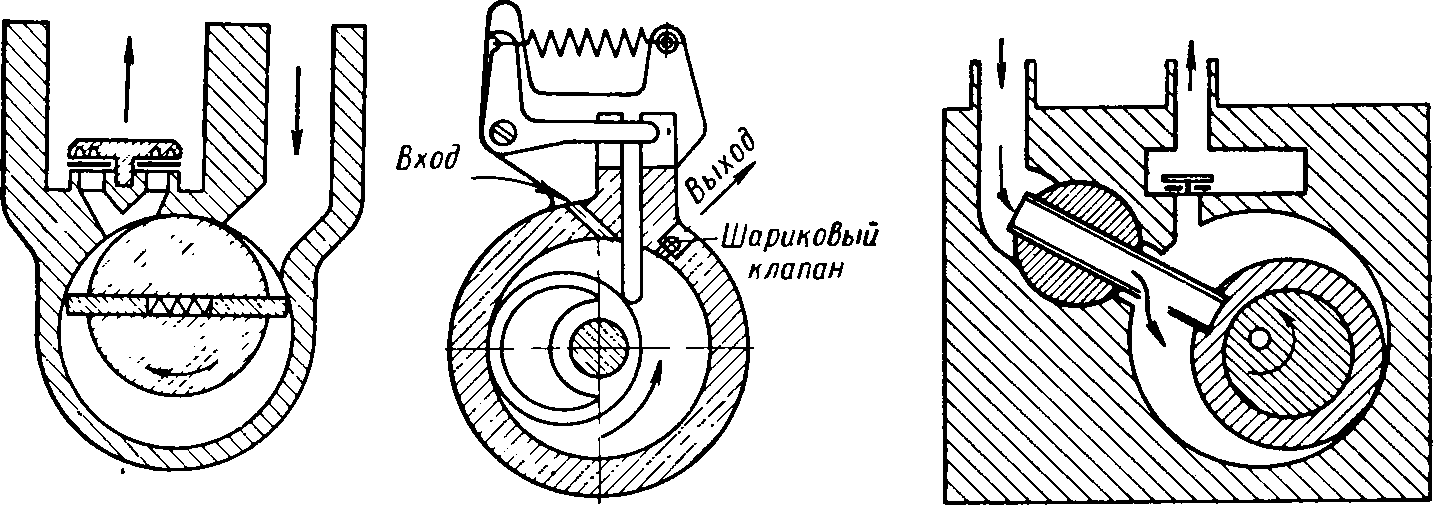
\includegraphics[width=0.85\linewidth]{pictures/rotor.png}
	\caption{Схемы вращательных масляных насосов: пластинчато-роторный (слева), пластинчато-статорный (по центру) и золотниковый (справа)}
\end{figure}

Среди вышеупомянутых трех видов масляных насосов наиболее распространены пластинчато-статорные насосы. В таком насосе в полости статора вращается цилиндрический ротор. Ось вращения ротора совпадает с осью полости статора, но не совпадает с осью самого ротора. Одна из образующих ротора все время скользит по поверхности полости статора. Пластина пружиной прижимается к ротору и совершает колебательное движение вверх-вниз в прорези статора. Пластина и ротор делят полость статора на два объема: расширяющийся и сжимающийся. Первый объем соединен с откачиваемой установкой, а второй -- с атмосферой (через клапан). Камера насоса помещена в бак с вакуумным маслом, которое предотвращает проникание воздуха через сочленения, а также смазывает ротор и уплотняет скользящие линии соприкосновения ротора со статором и пластиной. Таким образом, откачка происходит за счет диффузии молекул вещества в струю газа, которая затем выносится в форвакуумный насос.

\subsection*{Диффузионные насосы}

Для получения более высокого вакуума, чем вращательные насосы, используют диффузионные насосы. Работа этого типа насосов основана на диффузии молекул газа внутрь нанокапель масла (или в более ранних вариантах, ртути). Насос представляет собой цилиндрическую трубу, в основанию которой находится нагреватель, при помощи которого масло (в современных вариантах используется вазелиновое или силиконовое) нагревается до температуры кипения. Пары масла поднимаются по цилиндрической колонне и равномерно струятся через сопла, попадая в рабочий объем насоса под углом к стенкам корпуса. На стенках, охлаждаемых снаружи змеевиком с холодной водой, пары конденсируются и по стенке стекают обратно в кипятильник. Молекулы газа из откачиваемого объема диффундируют в струю пара и увлекаются ее вниз, где они удаляются форвакуумным насосом, присоединенным к патрубку диффузионного. 

\begin{figure}
	\centering
	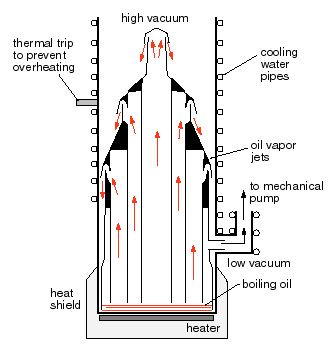
\includegraphics[width=0.45\linewidth]{pictures/diffusion_pump1.jpg}
	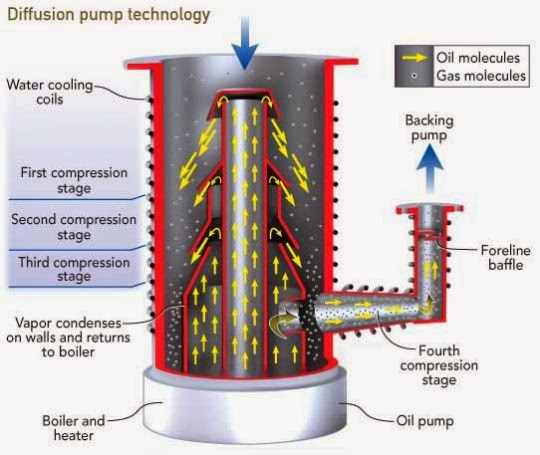
\includegraphics[width=0.45\linewidth]{pictures/diffusion_pump2.jpg}
	\caption{Схема диффузионного насоса}
\end{figure}

\subsection*{Турбомолекулярные и ионные вакуумные насосы}

Для создания сверхвысокого вакуума используются турбомолекулярные и ионные вакумные насосы. Турбомолекулярные насос состоит из большого количества вращающихся (роторов) и стационарных дисков (статоров). Молекулы газа, попадающие в камеру, ударяясь о поверхность ротора, получают дополнительную энергию, причем специальная форма ротора изменяет импульс молекул таким образом, чтобы они в преобладающем количестве направлялись в сторону статора. Многократные соударения с роторами приводит к существенному ускорению молекул на выходе из турбомолекулярного насоса, где они направляются в форвакуумный насос. Давление, достигаемое в камере, определяется скоростью вращения дисков. Главной технической трудностью при создании турбомолекулярных насосов является минимизация диссипативных сил между дисками и центральной осью насоса. \par 
Ионные насосы основаны на процессе ионизации молекул газ. Сильное электрическое поле вырывает электроны с поверхности анода, которые удерживаются магнитным полем внутри рабочего объема насоса. Внутри объема насоса происходят столкновения выбитых электронов с молекулами газа, приводящие к образованию молекулярных ионов. Эти ионы ускоряются электрическим полем, приобретают значительную кинетическую энергию и поверхность катода. Удар молекулярного иона в поверхность катода сопровождается возникновением вторичных эффектов, обусловленных распылением металла катода. В результате столкновения ионы газа частично проникают внутрь катода, также они могут отлететь и потом быть захваченными частицами металла, которые образовались в результате удара другого молекулярного иона в поверхность катода. Кроме того, частицы металла, осаждаясь на поверхности, создают поглощающую газ активную пленку. В итоге, подавляющее количество молекул газа осаждается на катоде, следовательно у ионных насосов нет выходящего потока. После длительного использования катод покрывается большим количеством дефектов, снижающих эффективность его работы.

\begin{figure}
	\centering
	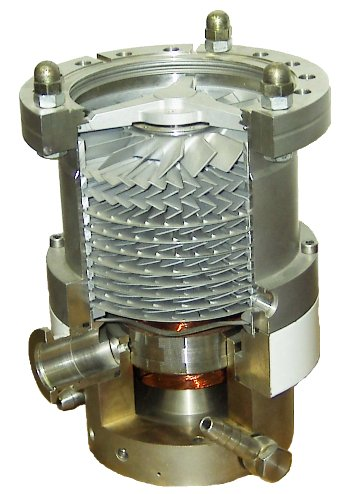
\includegraphics[width=0.3\linewidth]{pictures/turbomolecular_pump.jpg}
	\hspace{0.5cm}
	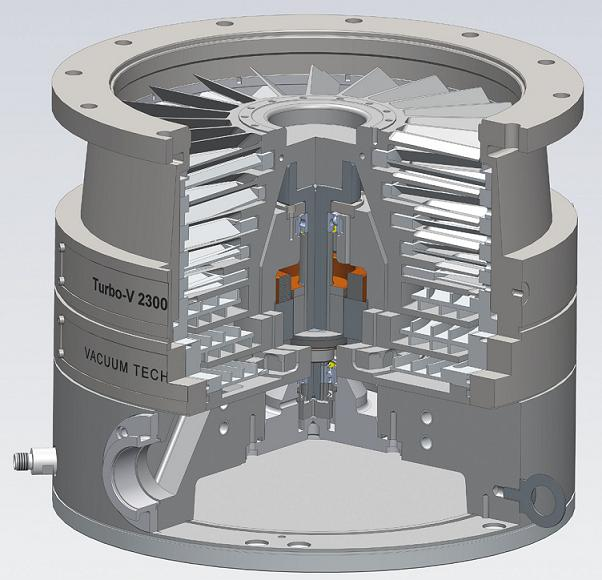
\includegraphics[width=0.3\linewidth]{pictures/turbomolecular_pump2.jpg}
	\hspace{0.5cm}
	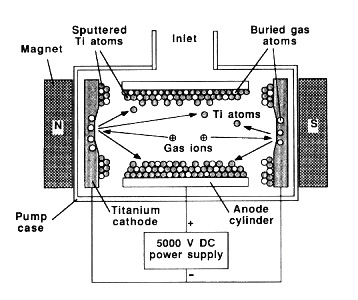
\includegraphics[width=0.3\linewidth]{pictures/ion_pump.jpg}
	\caption{Турбомолекулярный насос (слева и в центре); схема ионного насоса (справа)}
\end{figure}

\end{document}
